
%(BEGIN_QUESTION)
% Copyright 2006, Tony R. Kuphaldt, released under the Creative Commons Attribution License (v 1.0)
% This means you may do almost anything with this work of mine, so long as you give me proper credit

What does this table show?  What is its purpose?

$$\includegraphics[width=15.5cm]{i00550x01.eps}$$

\underbar{file i00550}
%(END_QUESTION)





%(BEGIN_ANSWER)

This table is called the {\it periodic table of the elements}, and it arranges all the known elements (unique types of atoms) in order of their atomic number, atomic weight, and chemical characteristics.

%(END_ANSWER)





%(BEGIN_NOTES)

The periodic table is the invention of Dmitri I. Mendeleyev, who demonstrated that different chemical substances exhibit a periodic recurrence of chemical properties (reactivities with other substances) when ordered according to their relative weight.  Mendeleyev's first table was based on atomic weight (mass) alone, and was not as accurate as modern tables whose order is based on atomic number.

%INDEX% Chemistry, basic principles: periodic table of the elements

%(END_NOTES)


